\section{Hardware}

There are two parts to this project, the software, algorithmic side of things, and the hardware on which this algorithm runs.
Here the details about the design and production of the PCB will be discussed, and explanations of why certain decisions were made.

\subsection{Schematic}
Before producing the PCB design the system was designed in gEDA Schematic software.
In order to keep the design easy to maintain hierarchy was used, and the system split into multiple sections.
These sections are discussed below.

\begin{figure}[H]
	\centering
	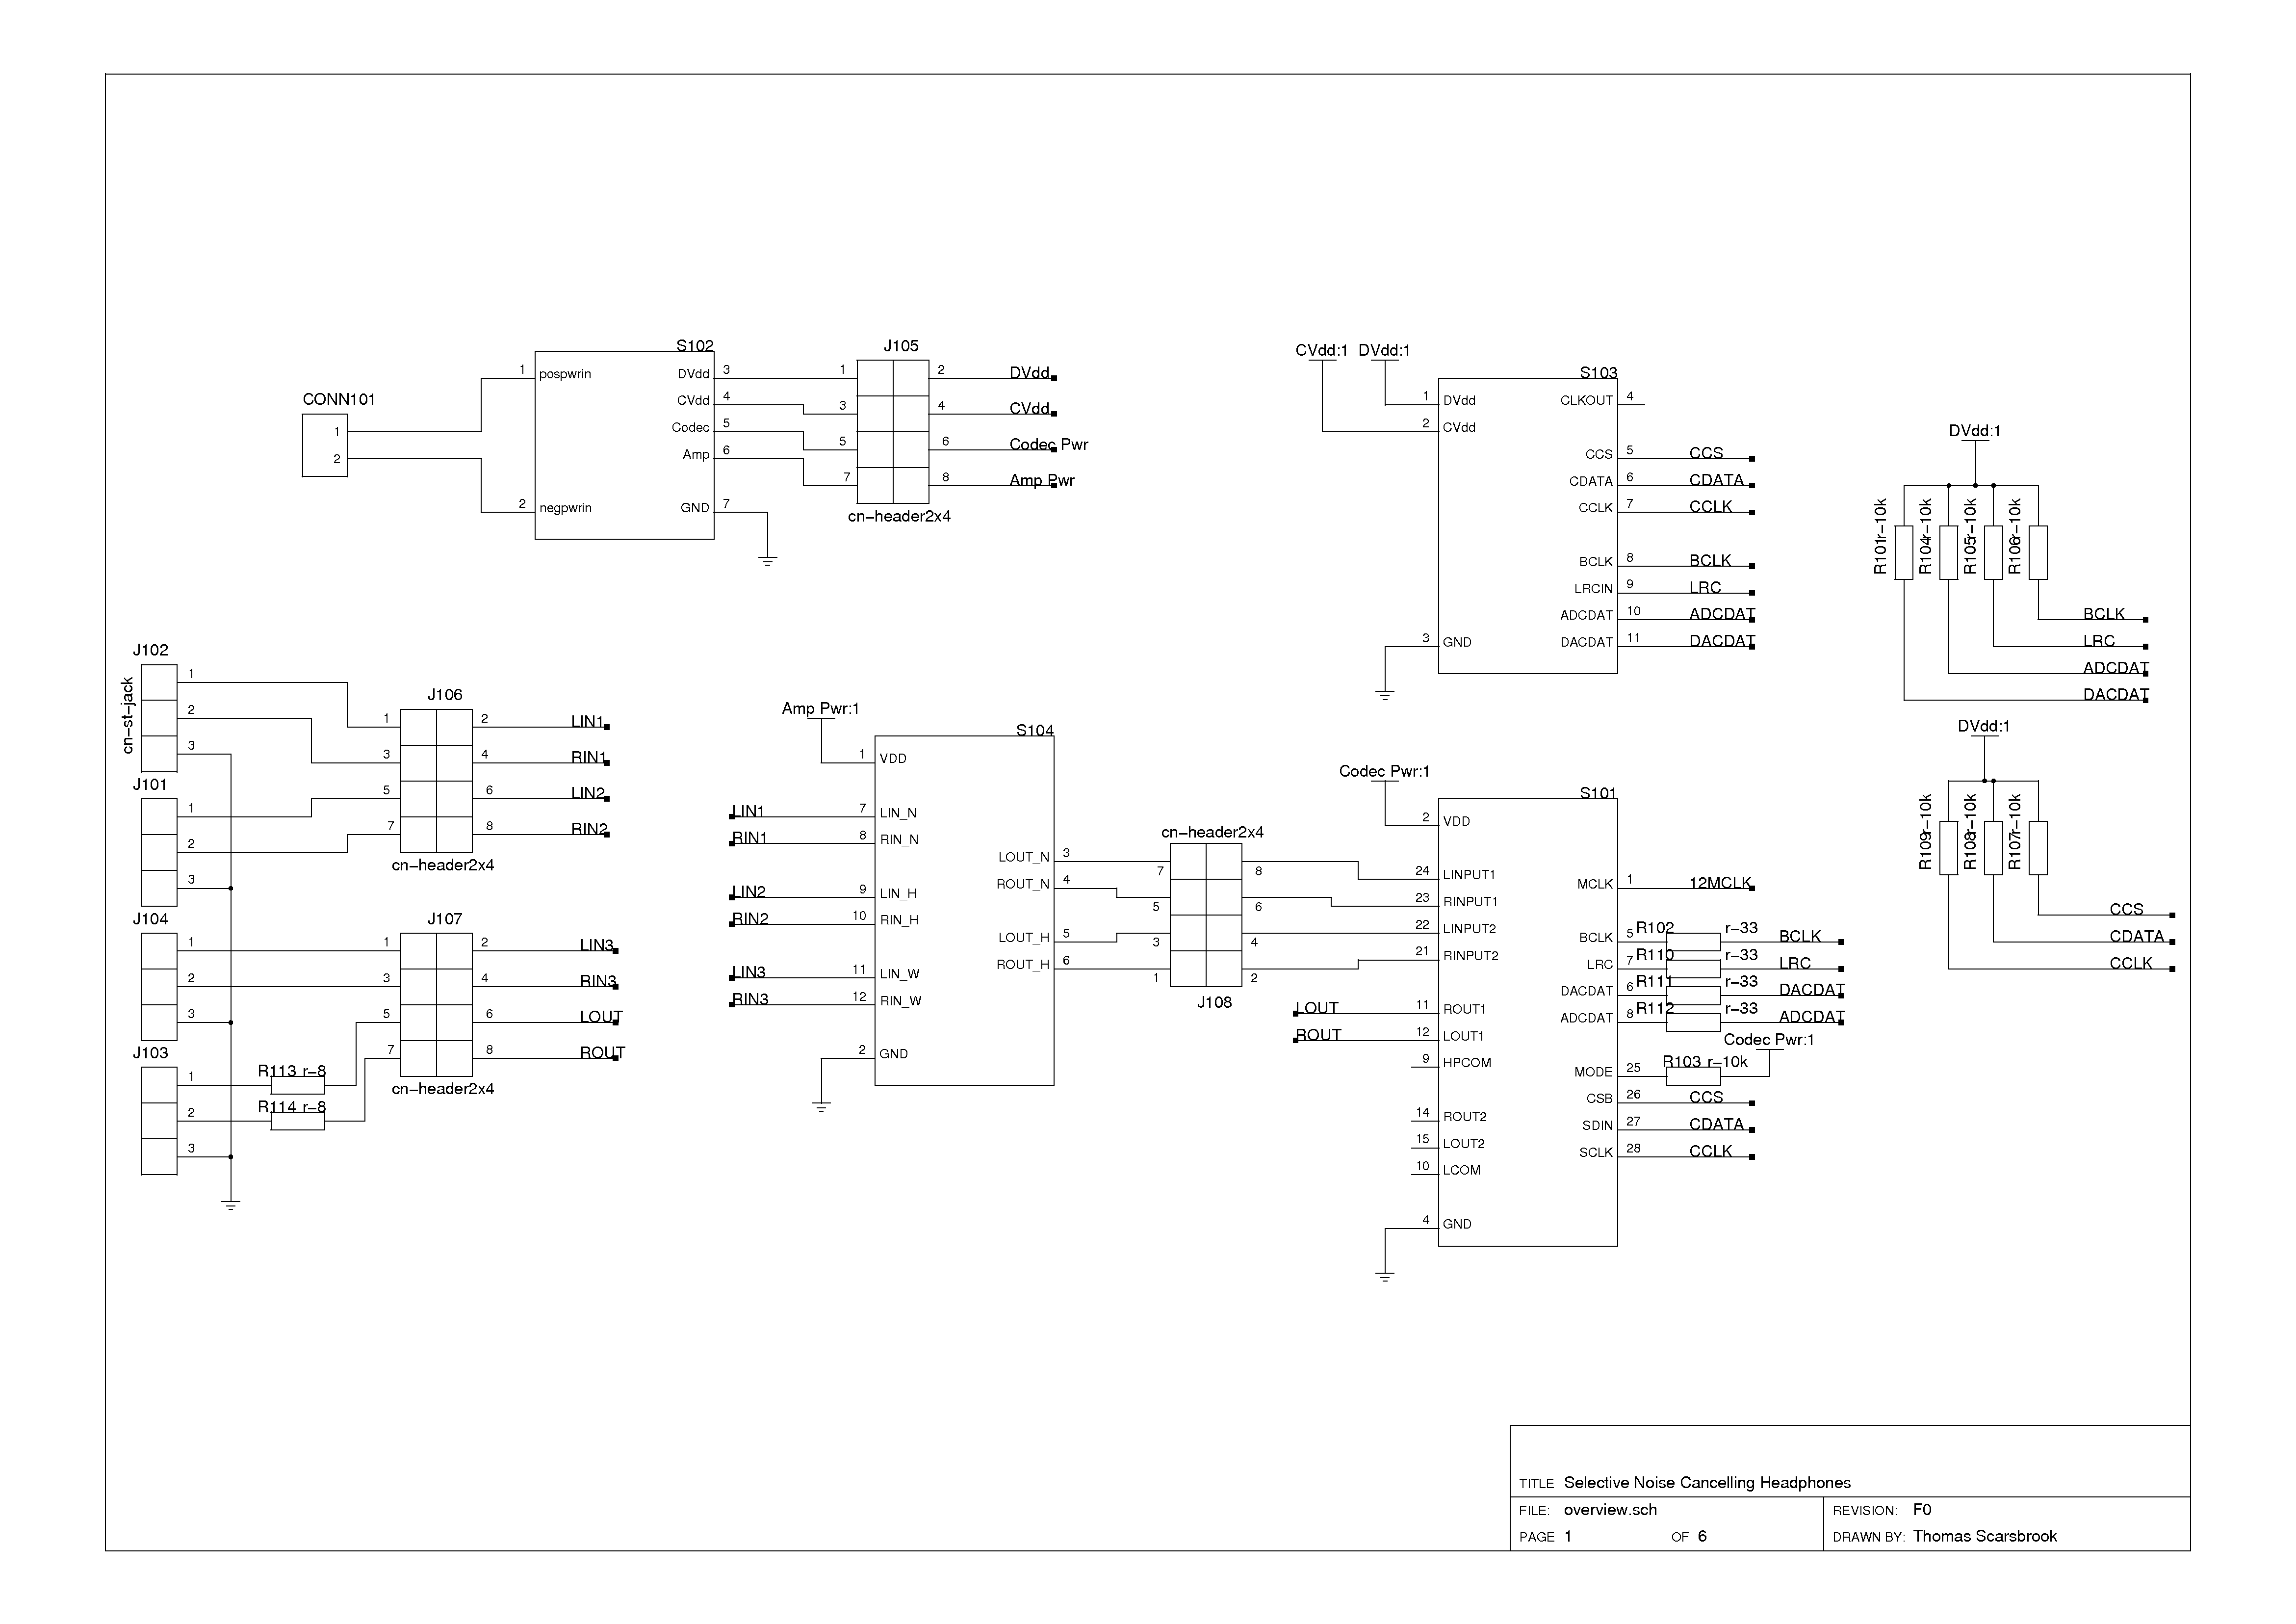
\includegraphics[width=\textwidth]{./img/overview.png}
	\caption{The top level schematic}
	\label{fig:overviewsch}
\end{figure}

\subsubsection{DSP}
At the heart of the project is the digital signal processor.
This is the part that achieves all the calculations required by the cancelling algorithm.

\subsubsection{Codec}
The DSP is unable to read analogue signals, and therefore requires the analogue signals from the microphones involved to be sampled by an external device.
This is where the codec comes in.
Wolfson MicroElectronics WM8988 was chosen for four reasons.
Firstly it supports a communication protocol supported by the McBSP system on the DSP.
This allows the configuration of the codec to be set easily, along with the acquisition and outputting of audio samples.
Secondly the codec provides two stereo inputs, which is what is required for this project, one for the noise signal, one for the heard/demanded signal.
On top of this the codec has a output with a headphone driver, meaning that no further electronics is required between the codec and the headphones, so impedance matching is not an issue.
Finally, the codec supported sampling frequencies suitable for the full spectrum of human hearing, meaning high frequency components would not evade being cancelled.
\\
\\
However, the codec could not function purely by itself, it requires some surrounding electronics.
Some basic resistors and capacitors are required on the codecs I/O ports, but the most significant piece of supporting electronics it required was a clock.
This clock was required so it could generate the appropriate timings for the sampling frequencies and the communications with the DSP.

\begin{figure}[H]
	\centering
	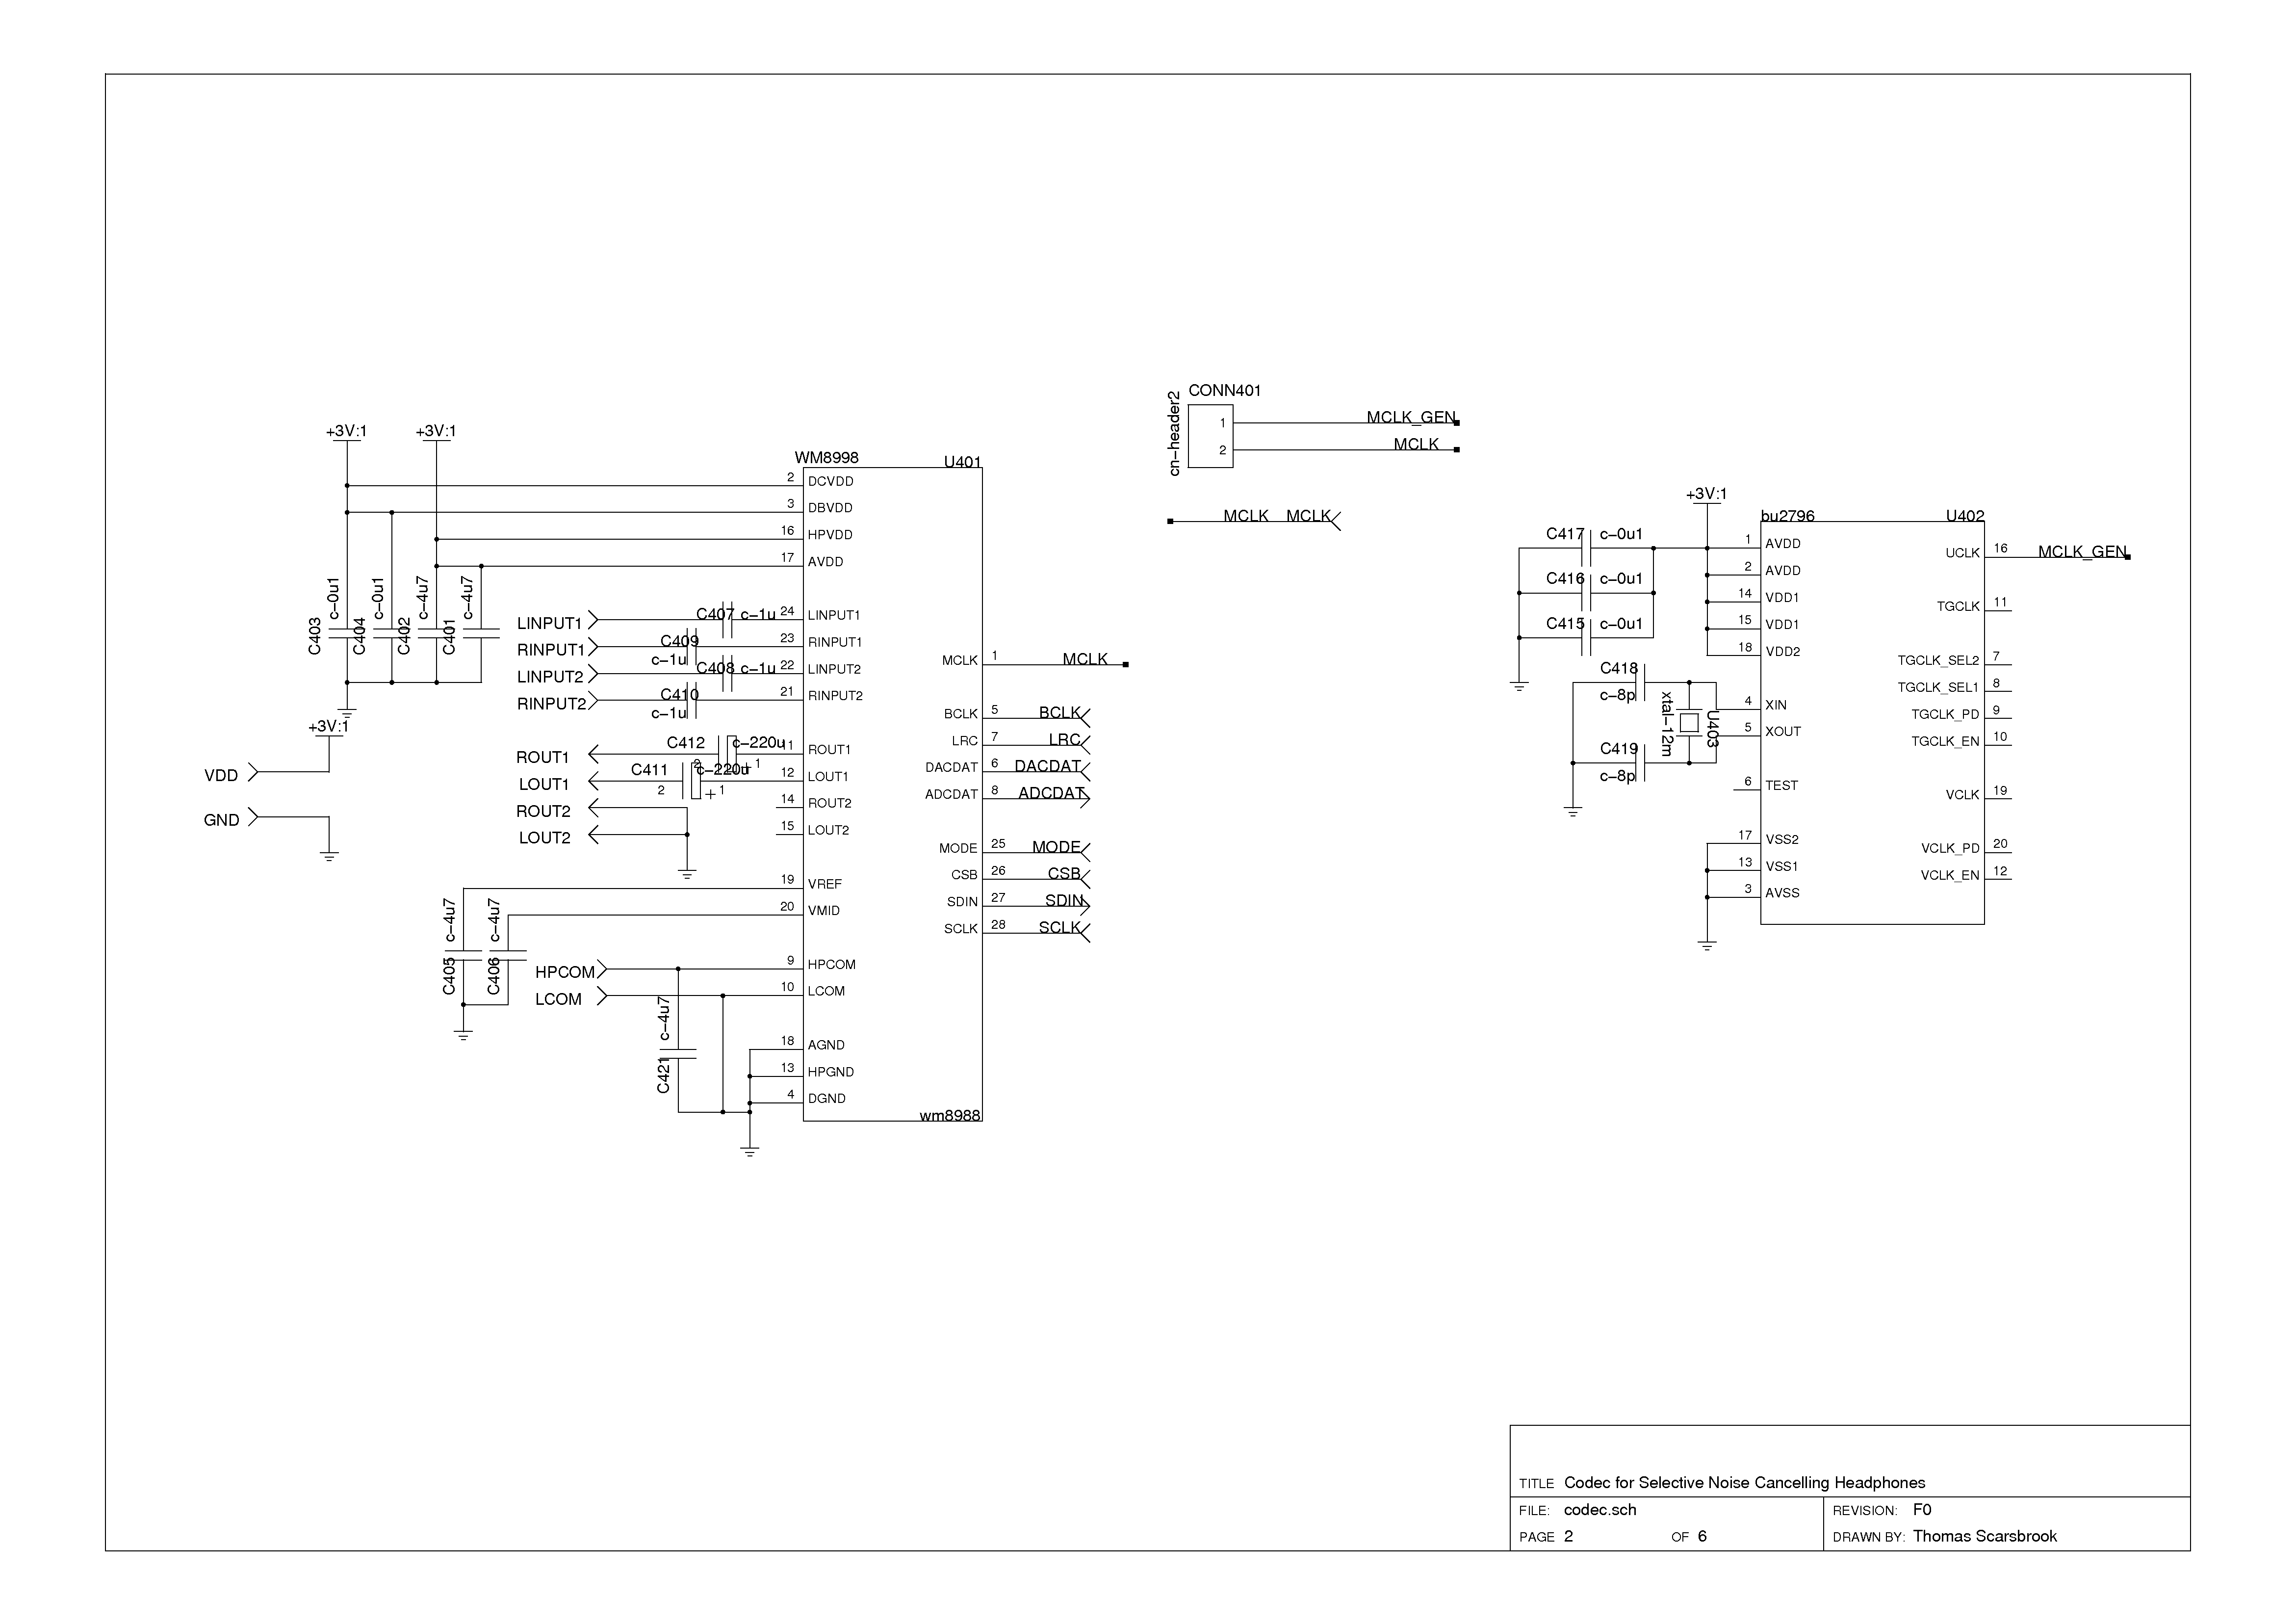
\includegraphics[width=\textwidth]{./img/codec.png}
	\caption{The schematic for the codec}
	\label{fig:codecsch}
\end{figure}

\subsubsection{Analogue}
Before the codec the signal needs some conditioning.
If any signal received were to be passed into the codec it could contain components at too high a frequency, these need to be removed to prevent aliasing.

\begin{figure}[H]
	\centering
	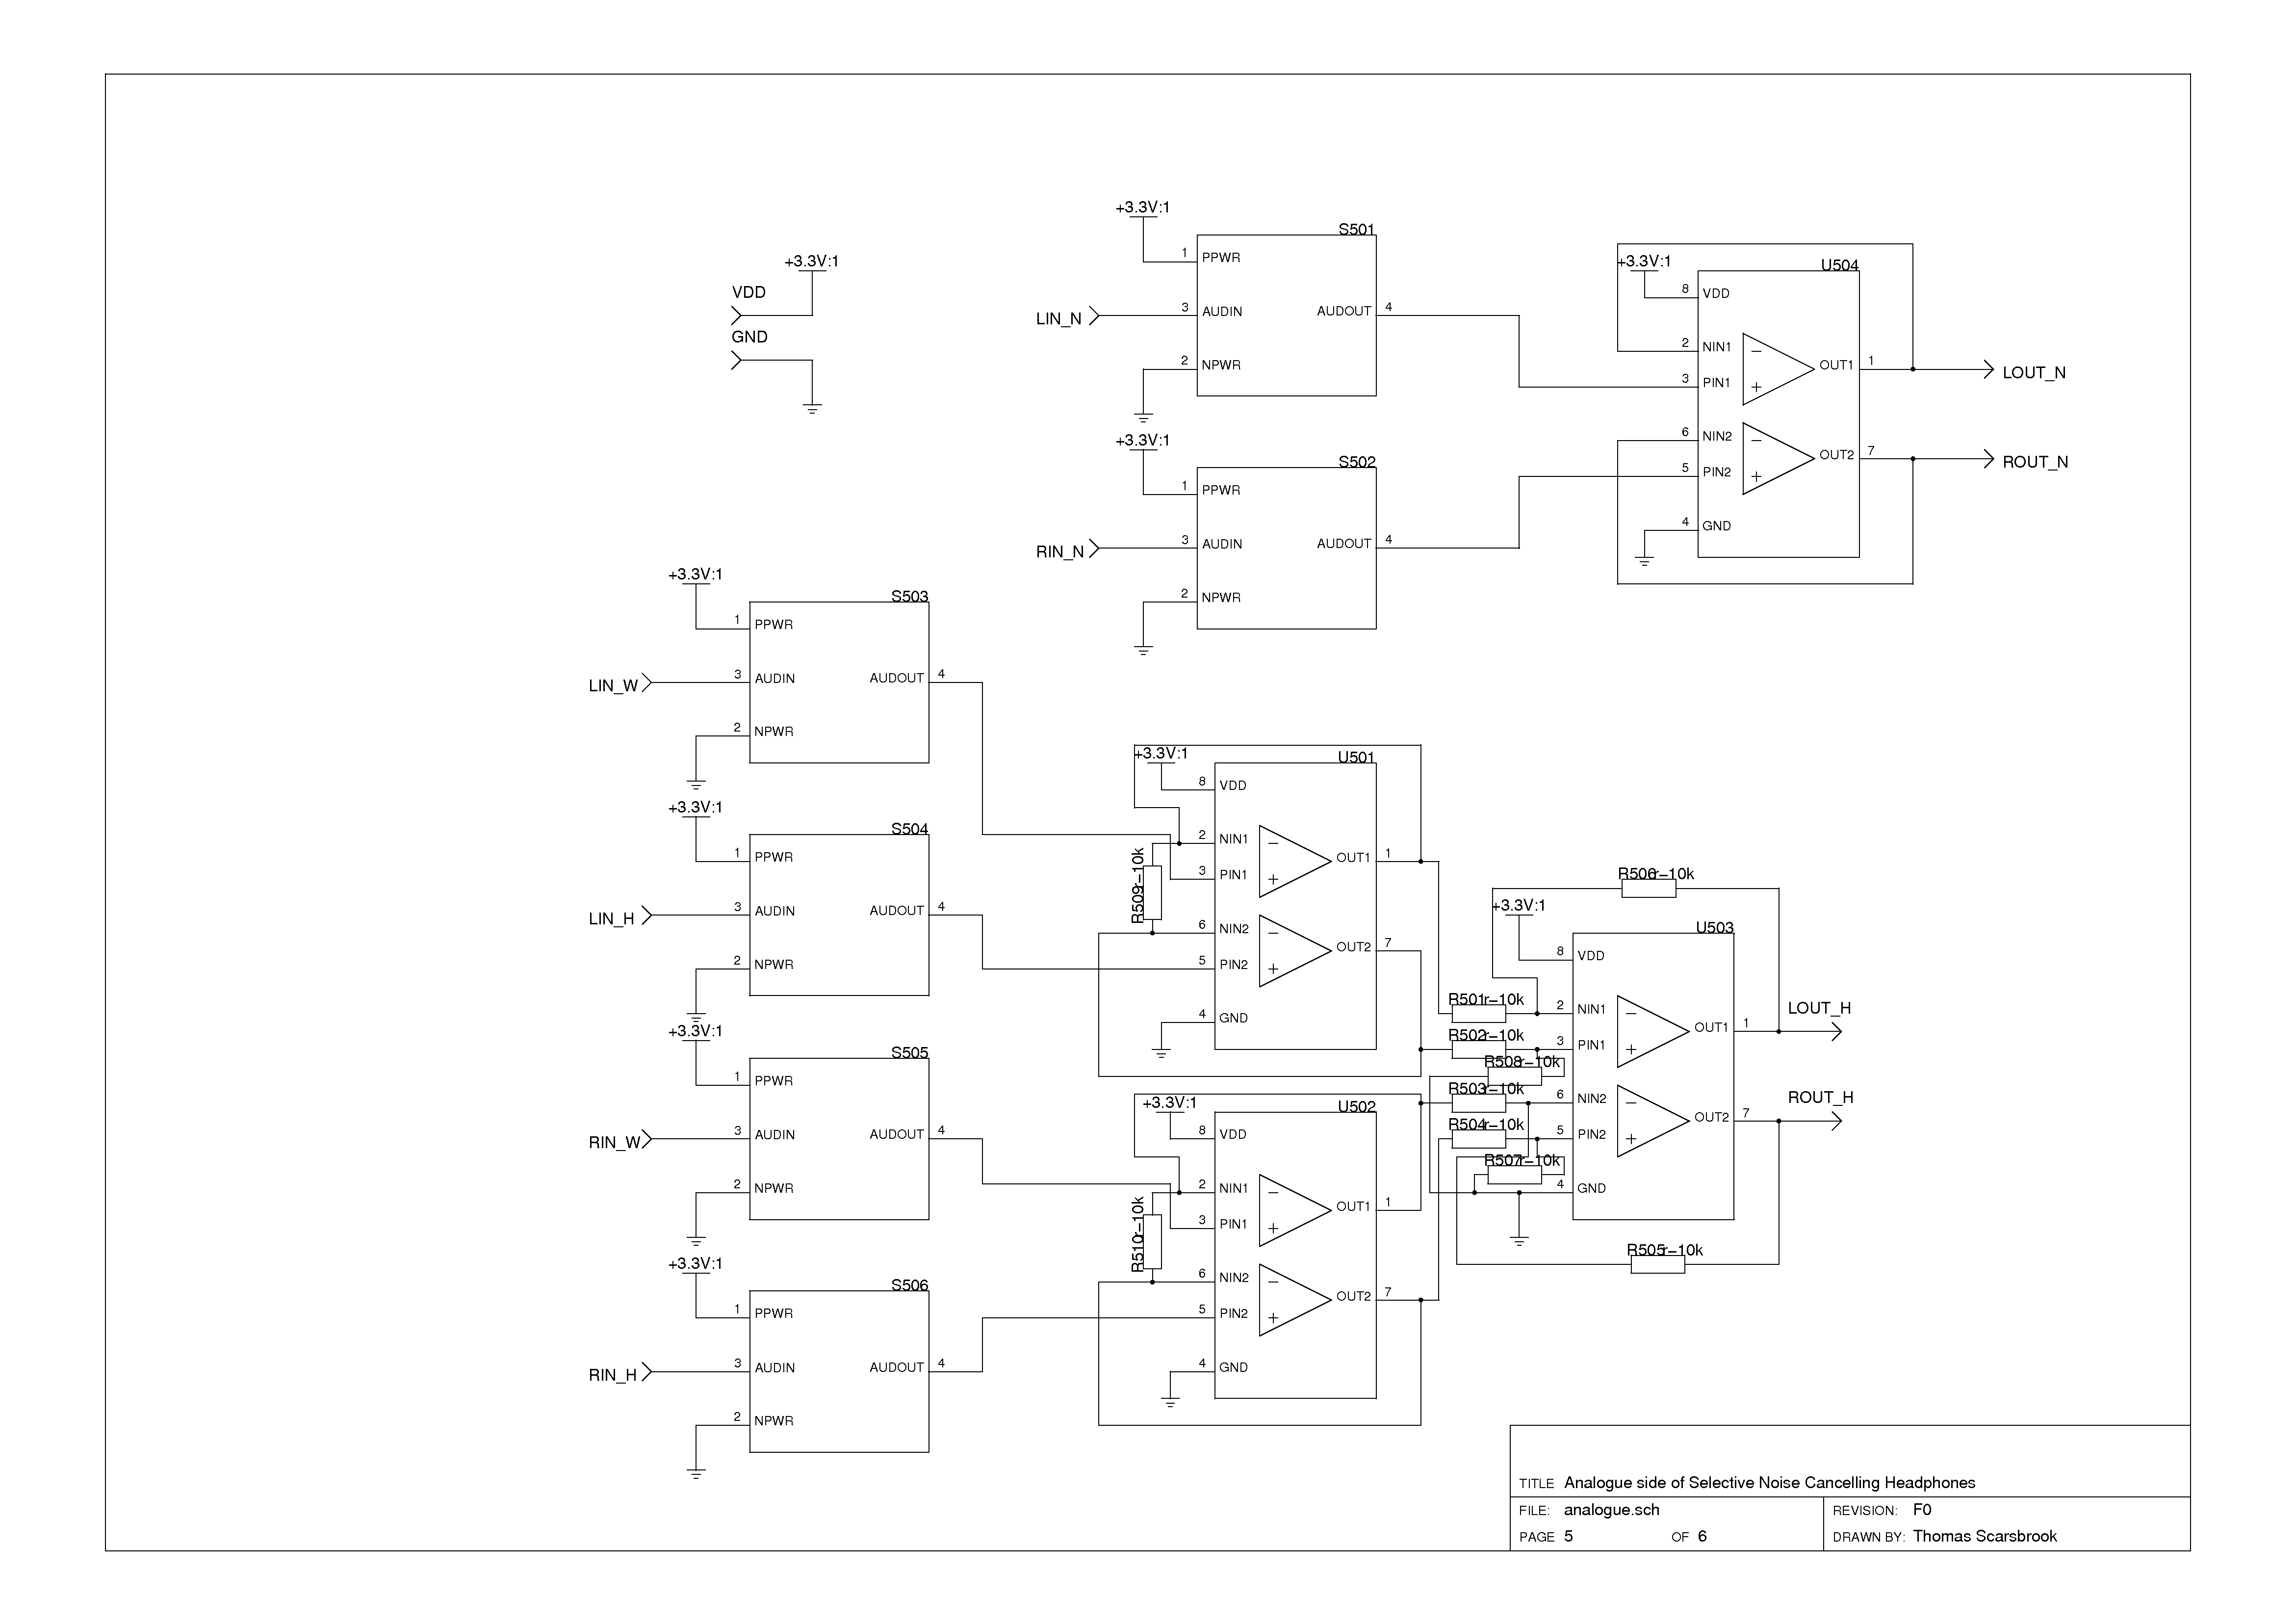
\includegraphics[width=\textwidth]{./img/analogue.png}
	\caption{The schematic of the analogue portion of the project}
	\label{fig:analoguesch}
\end{figure}

\noindent This portion of the design is then further split into two parts, the instrumentation amplifier and the signal conditioning.
The instrumentation amplifier takes in the noise and the optional demanded signal, and sums the two together.
This choice of amplifier was based on a few requirements.
The inputs from the microphones on the headphones require the amplifier to have a large input impedance.
Using a naive summing amplifier would result in a much lower input impedance due to the mixing resistors.
In contrast, the demanded input is likely to be from an MP3 player or similar, which will provide a low output impedance due to being designed to connect direct to, and drive headphones.
As such this input does not require the same high impedance from the amplifier, however the signal is not harmed by it.
Providing this high impedance also allows microphones to be connected and still serve equally well.
The second requirement of the amplifier is that it must sum the signals together with minimal distortion to the heard signal.
Adding distortion would result in sub-optimal cancellation, due to the actual heard signal not being known.
The instrumentation amplifier is a difference amplifier, as such one of its input is affected by a phase shift of 180$^{\circ}$.
As the demanded signal has no specific requirement for phase being maintained, this signal is the one that gets inverted.
\\
\\
Signal conditioning is required in order to prevent aliasing occurring when the input signals are sampled.
In order to accomplish this a naive low-pass filter was used, as show in figure \ref{fig:sigcondsch}.
This design was chosen due to its simplicity to implement and minimal power draw, whilst still maintaining a high input impedance and suitable roll-off.

\begin{figure}[H]
	\centering
	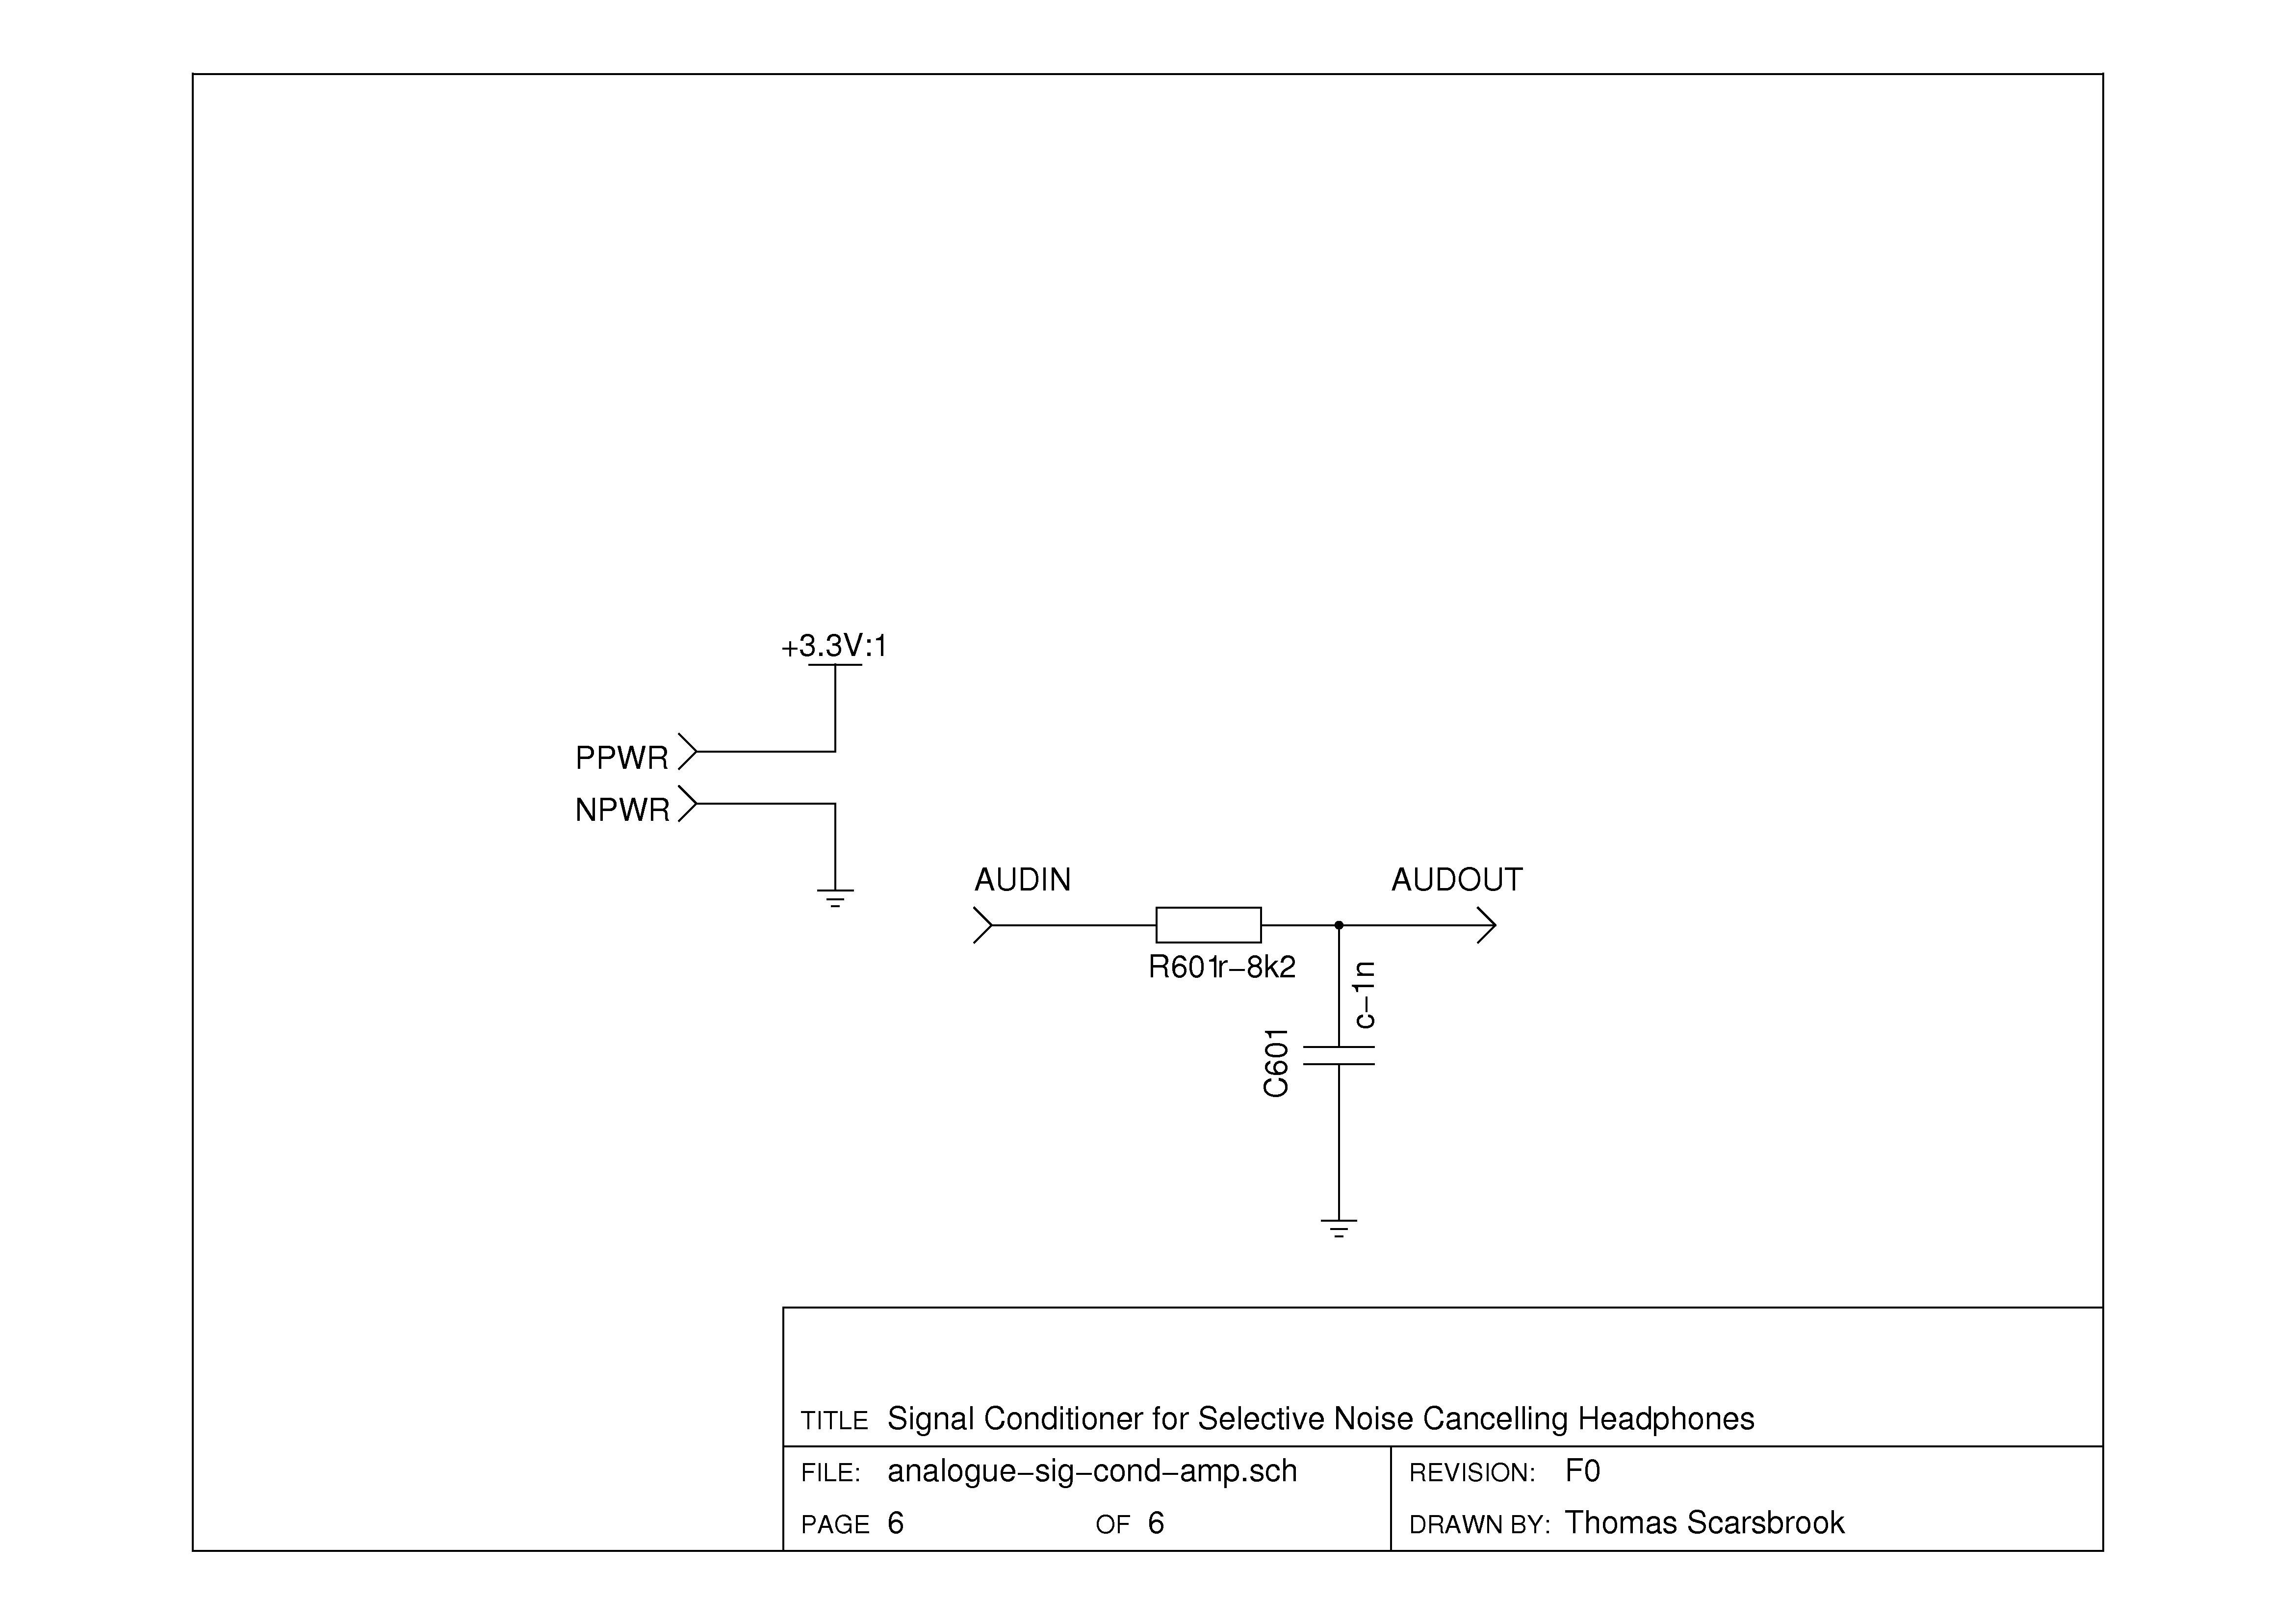
\includegraphics[width=\textwidth]{./img/analogue-sig-cond-amp.png}
	\caption{The signal conditioning amplifier schematic}
	\label{fig:sigcondsch}
\end{figure}

\noindent This design was tested through the use of a signal generator and digital oscilloscope.
The results can be seen below.

\subsubsection{Power}
One key part of any electronic system is it needs some form of power supply, and this project is no exception.
Multiple voltage rails were required, due to the DSP requiring a core voltage level as well as a second level for I/O.
The voltage level required by the codec and the amplifiers was the same as the one required by the DSP I/O, simplifying the design.

\begin{figure}[H]
	\centering
	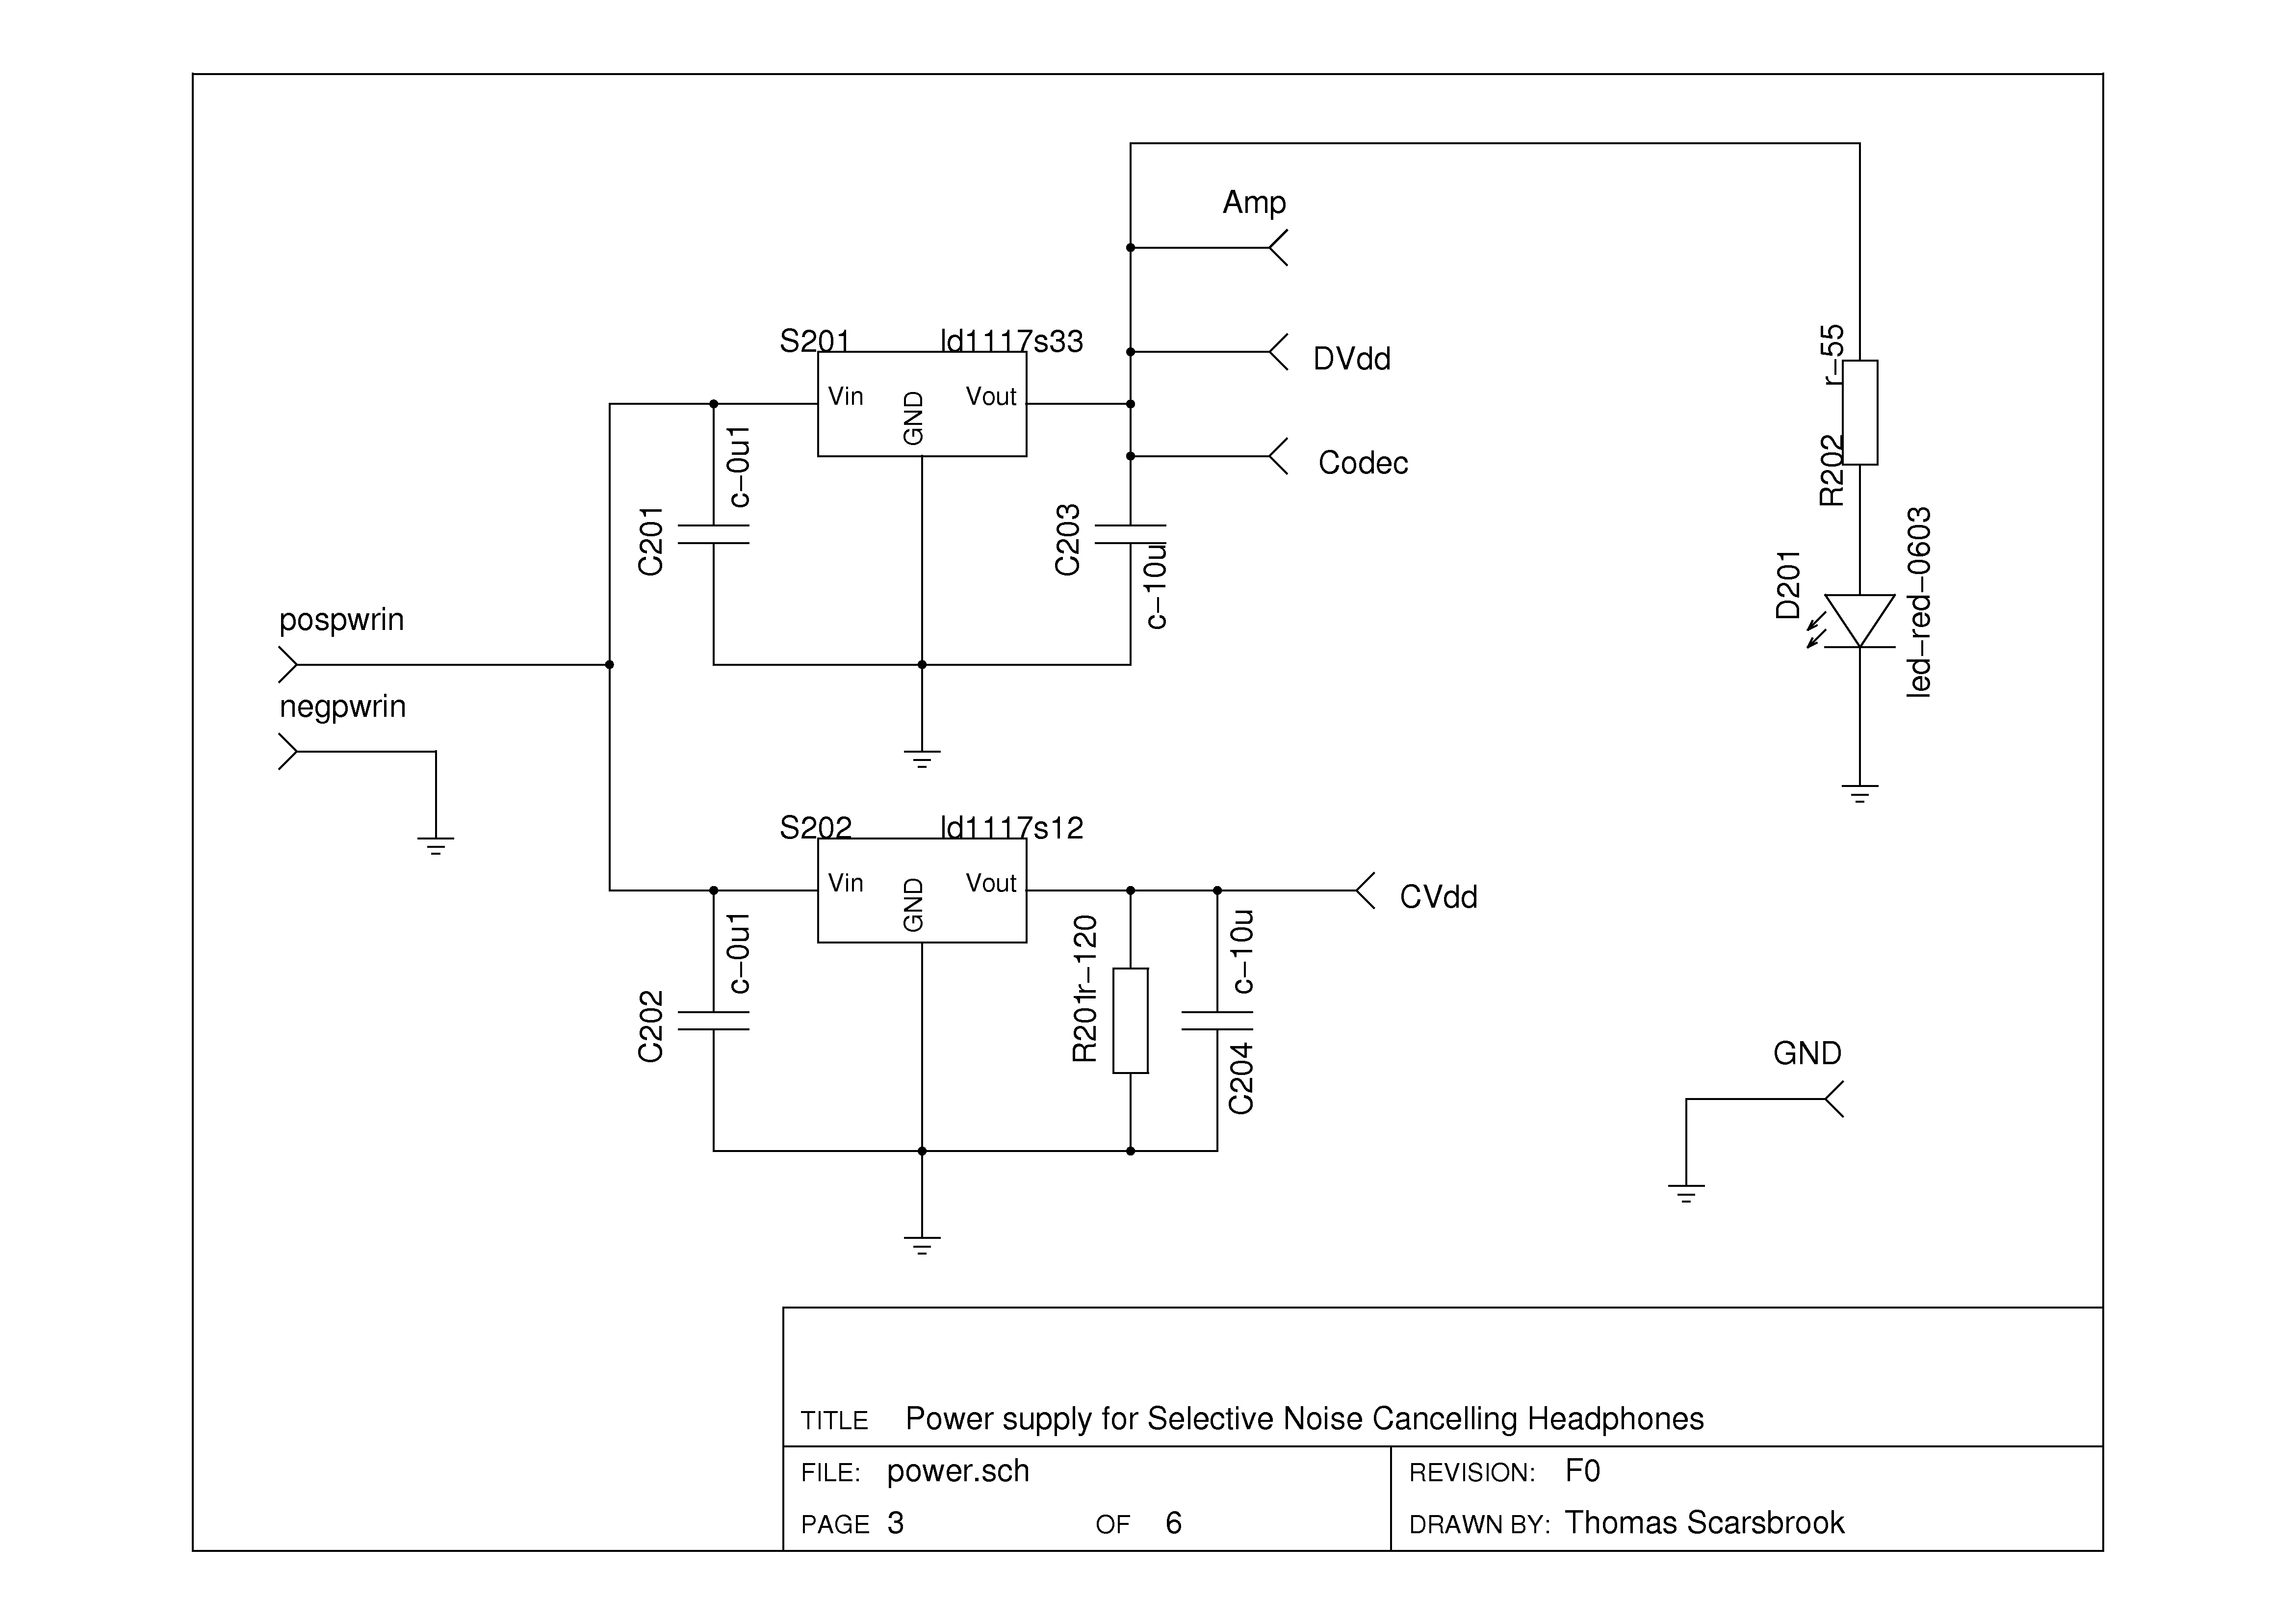
\includegraphics[width=\textwidth]{./img/power.png}
	\caption{The schematic of the power regulation for the projects PCB}
	\label{fig:powersch}
\end{figure}

\noindent In order to account for this two voltage regulators were obtained, one providing the 3.3V required by the DSP I/O and other circuitry, and the other providing the 1.2V required by the DSP core.
Both of these regulators were capable of providing 1.2A, which is in excess of the current requirements of the devices.
An LED was connected to the 3.3V rail to show when power was being provided, regardless of state of the rest of the system.

\begin{table}[H]
	\centering
	\begin{tabular}[c]{| l | c |}
		\hline
		\multicolumn{2}{|l|}{3.3V rail}\\
		\hline
		Component	& Draw (mA)	\\
		\hline
		DSP I/O		& 75	\\
		Codec		& 35.1	\\
		Clock Generator	& 160.6	\\
		Amplifiers	& 2	\\
		\hline
		Total		& 272.7	\\
		\hline
		\hline
		\multicolumn{2}{|l|}{1.2V rail}\\
		\hline
		Component	& Draw (mA)	\\
		\hline
		DSP core	& 625	\\
		\hline
		Total		& 625	\\
		\hline
	\end{tabular}	
	\caption{The current requirements of the various components in the circuits}
	\label{tab:pcbcurrentdraw}
\end{table}

\subsection{PCB}
The PCB was designed in gEDA PCB.

\begin{itemize}
	\item Two ground planes
	\item Decoupling capacitors
	\item Two layers
	\item QFP instead of BGA
	\item Segmentation
	\item Debug Headers
	\item Audio I/O
\end{itemize}

\begin{figure}[H]
	\centering
	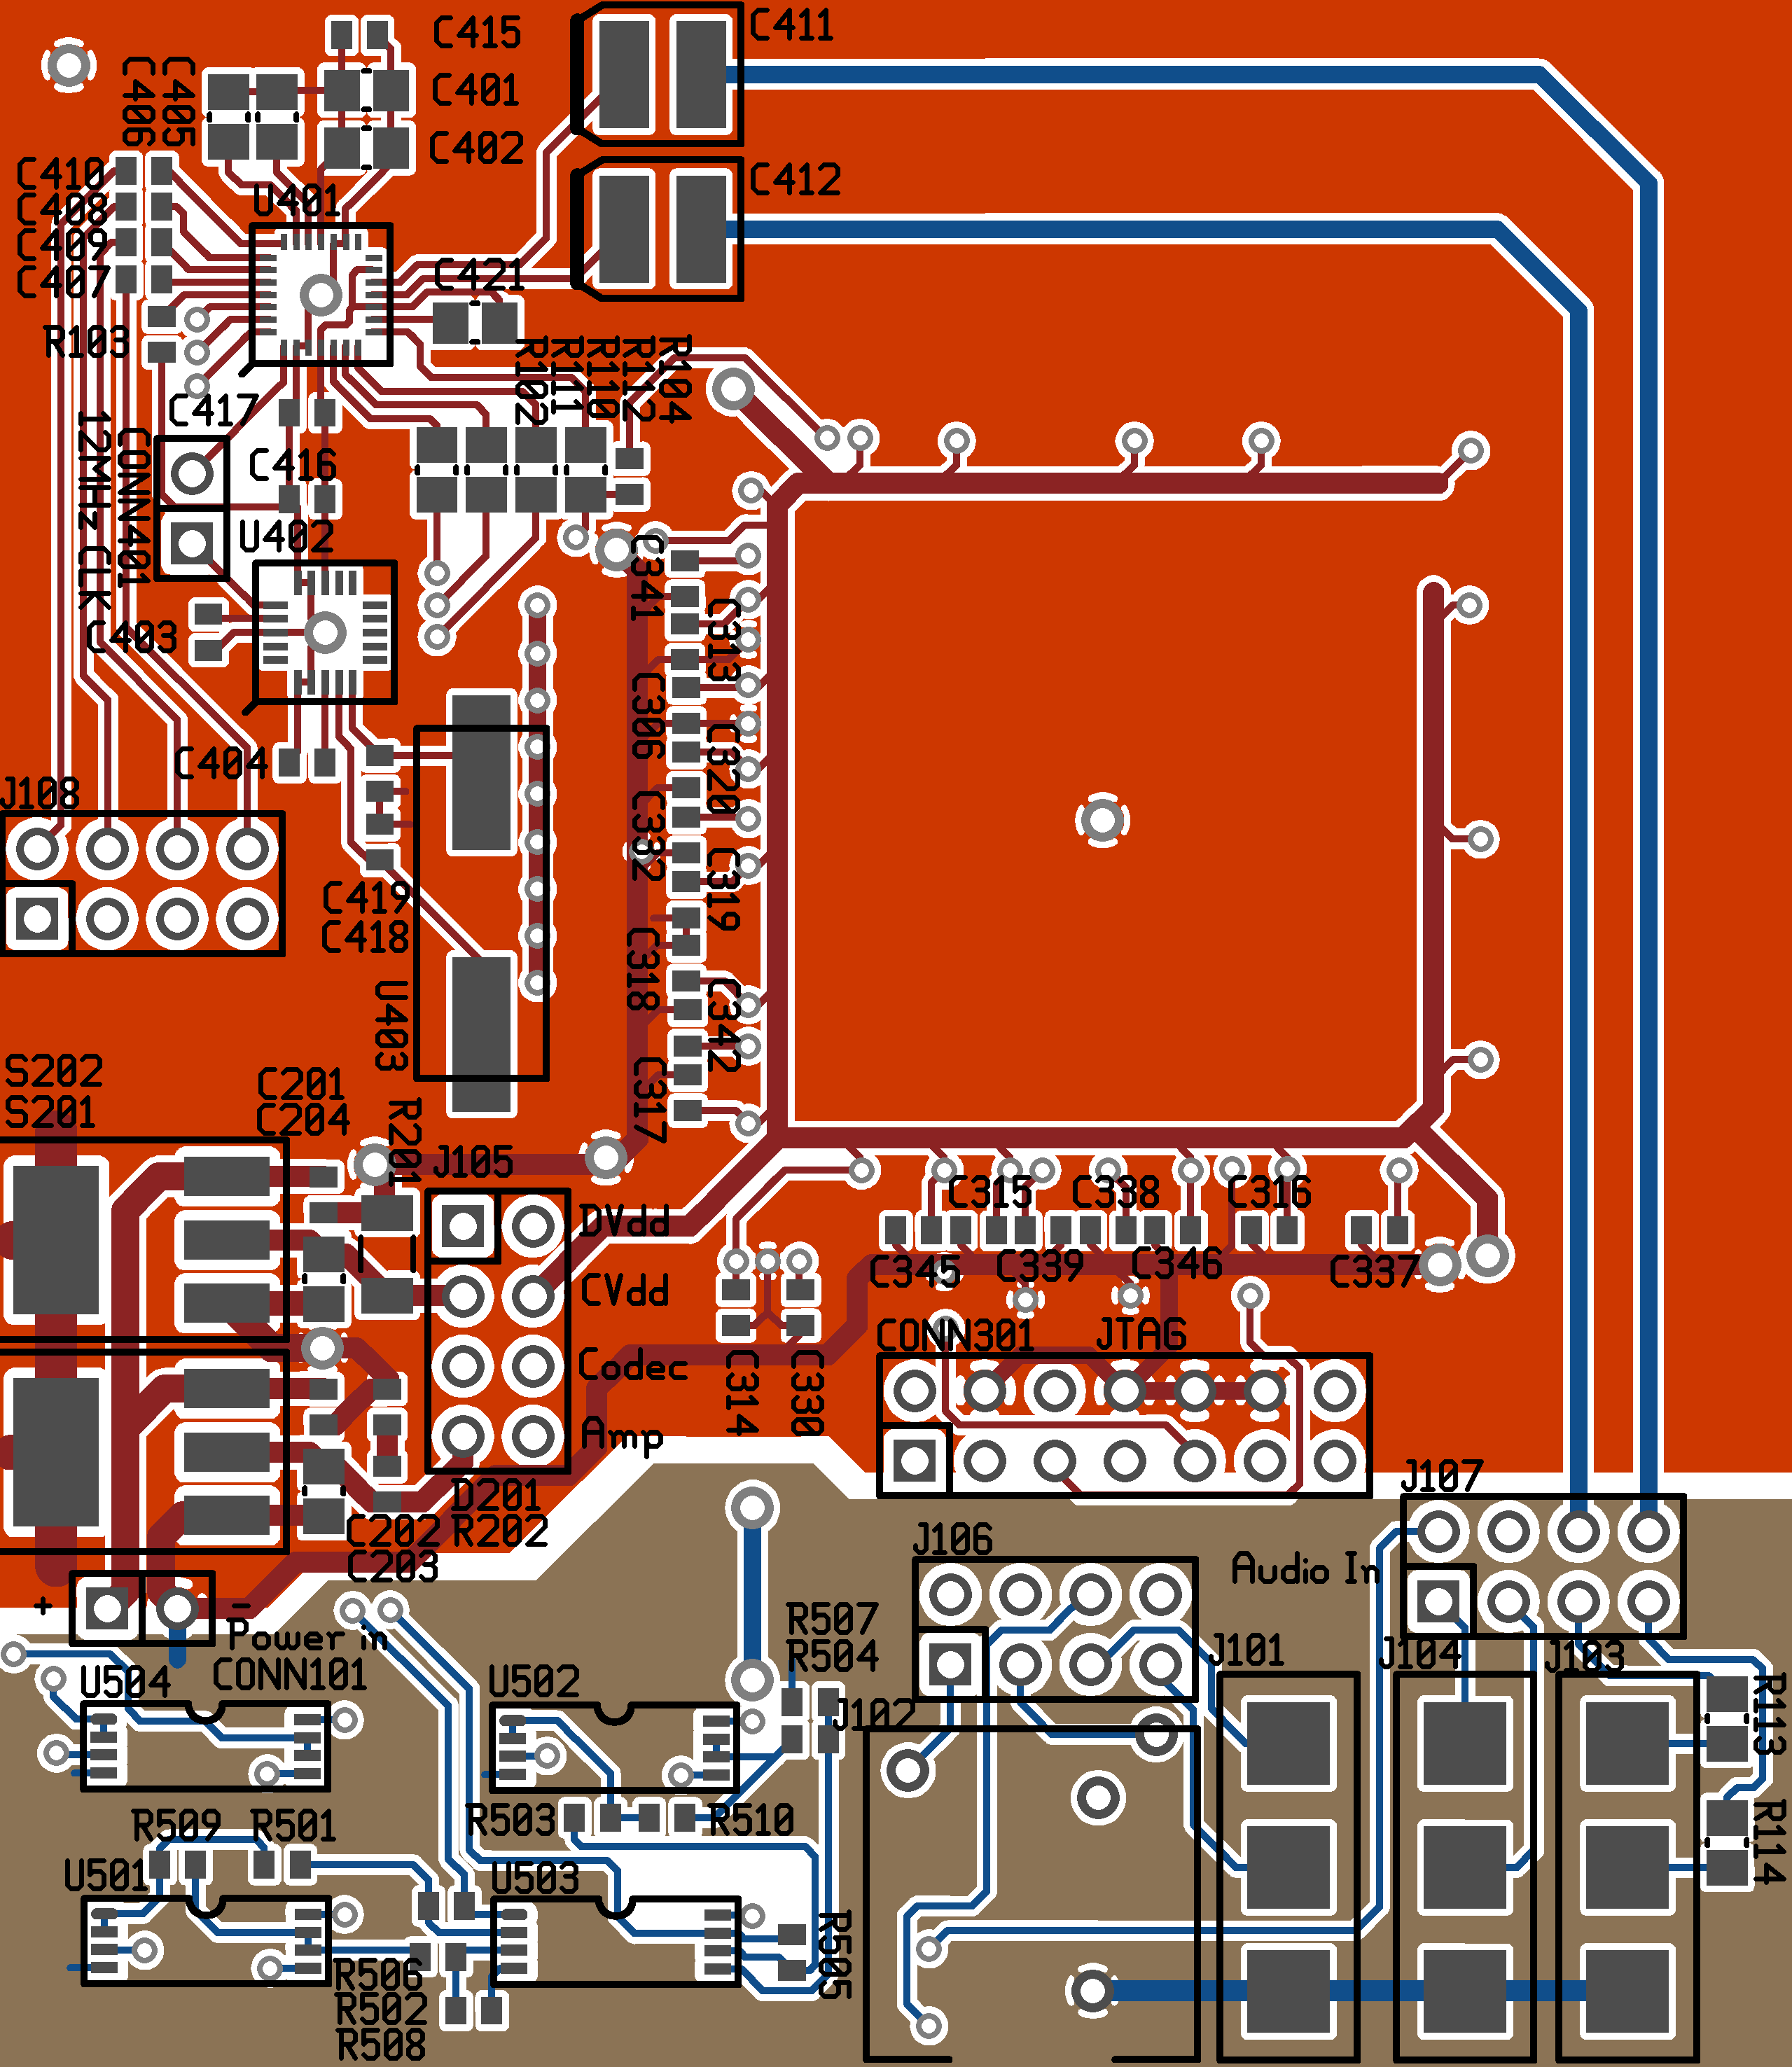
\includegraphics[width=280px]{./img/overview_top.png}
	\caption{The top side of the PCB}
	\label{fig:pcbtop}
\end{figure}
\begin{figure}[H]
	\centering
	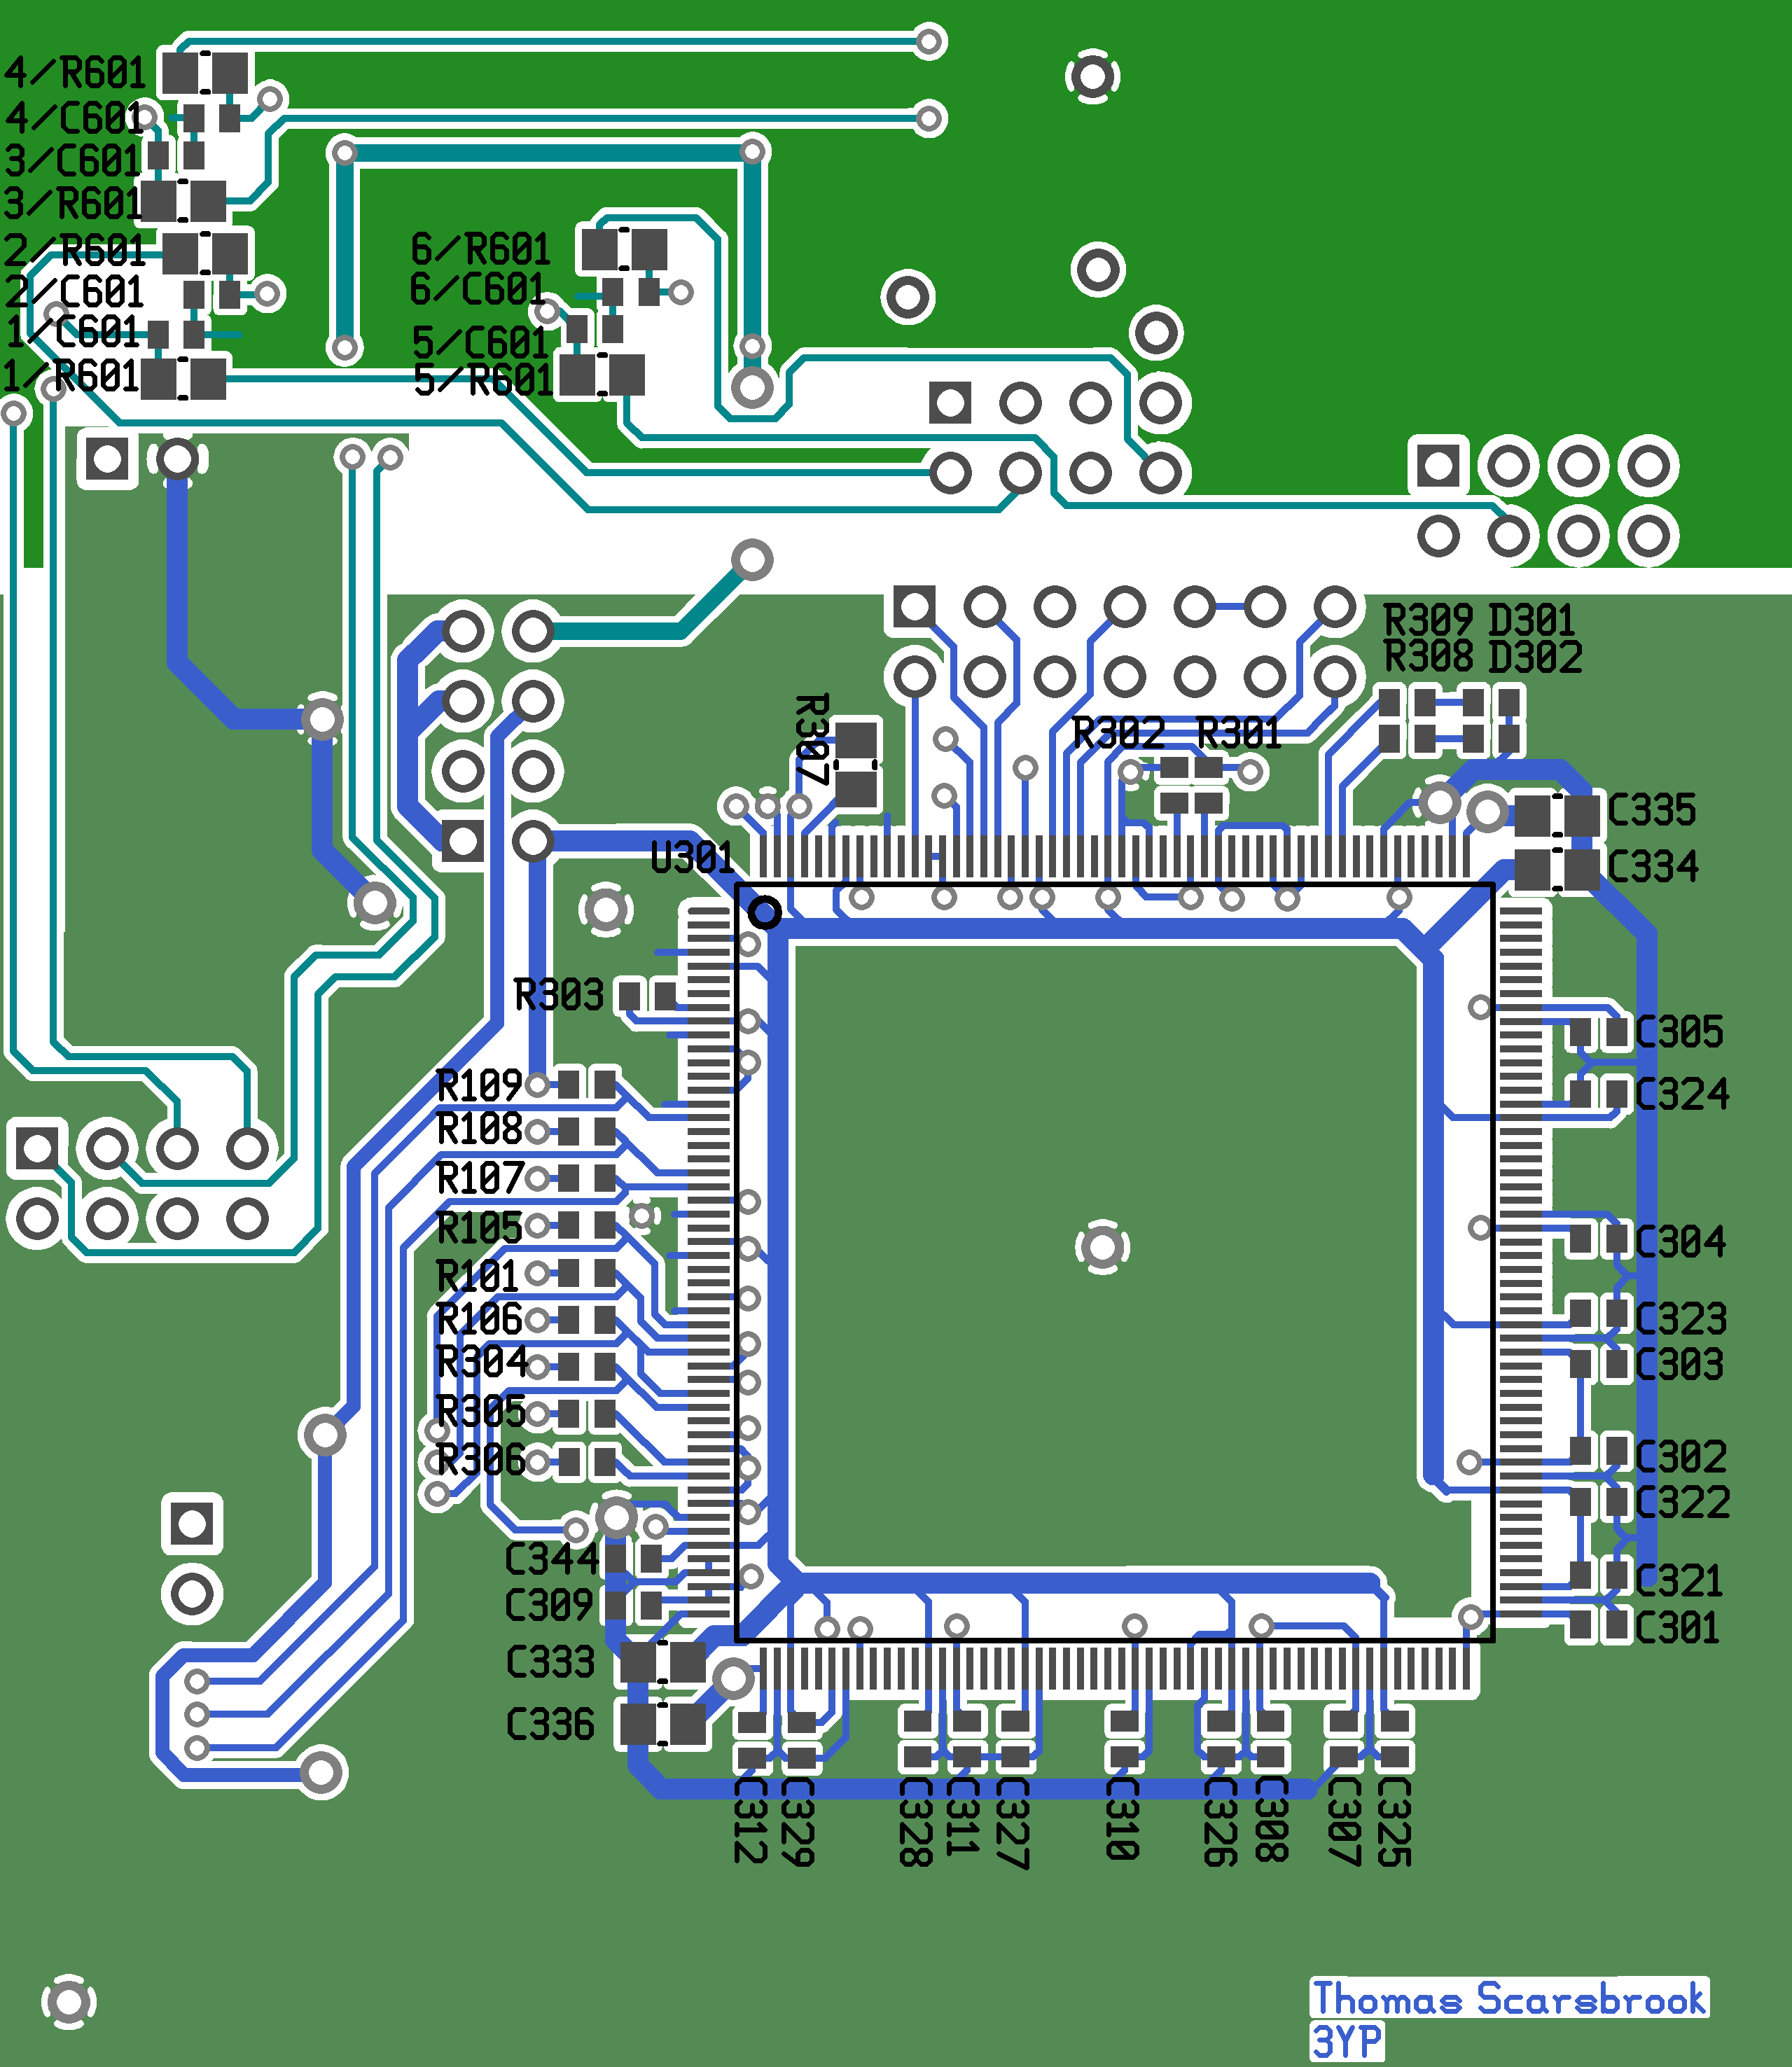
\includegraphics[width=280px]{./img/overview_bottom.png}
	\caption{The bottom side of the PCB}
	\label{fig:pcbbottom}
\end{figure}
